\documentclass[10pt,a4paper]{article}
\usepackage[margin=0.7in]{geometry}
\usepackage{multicol}
\usepackage{amsmath}
\usepackage{tikz}
\usepackage{enumitem}
\usepackage{titlesec}
\usepackage{booktabs}
\usepackage{fontspec}

% Compact formatting
\setlength{\columnsep}{0.7cm}
\setlength{\parindent}{0pt}
\setlength{\parskip}{0.12cm}
\titlespacing{\section}{0pt}{0.4cm}{0.15cm}
\titlespacing{\subsection}{0pt}{0.25cm}{0.08cm}
\titlespacing{\subsubsection}{0pt}{0.2cm}{0.05cm}

% Custom section style
\titleformat{\section}{\large\bfseries}{}{0em}{}
\titleformat{\subsection}{\normalsize\bfseries}{}{0em}{}
\titleformat{\subsubsection}{\normalsize\bfseries\itshape}{}{0em}{}

\begin{document}

\begin{center}
{\LARGE \textbf{Elasticity of Demand and Supply}}\\[0.15cm]
{\normalsize \textit{Topic 3: Measuring Responsiveness in Economics}}\\[0.15cm]
\hrule
\end{center}
\vspace{-0.3cm}

\begin{multicols}{2}
\footnotesize

% ============================================================================
% PART 1: DEFINITIONS AND CORE CONCEPTS
% ============================================================================
\section*{1. Definition and Conceptual Foundation}

\subsection*{What is Elasticity?}
\textbf{Elasticity} is a measure of \textbf{responsiveness} -- the degree to which one economic variable changes in response to a change in another variable, \textit{ceteris paribus}. In simple terms, it answers: ``How much does quantity demanded/supplied react when price or income changes?''

\textbf{Why Elasticity Matters:}
\begin{itemize}[leftmargin=*,nosep]
    \item Businesses use it to set prices optimally (will a price hike raise or lower total revenue?).
    \item Governments use it to design taxes (will a sugar tax reduce consumption significantly?).
    \item Policymakers use it to predict effects of subsidies, trade tariffs, or minimum wages.
\end{itemize}

\textbf{General Formula:}
\[
\text{Elasticity} = \frac{\% \text{ Change in Quantity}}{\% \text{ Change in Determinant}} = \frac{\Delta Q / Q}{\Delta X / X} = \frac{\Delta Q}{\Delta X} \cdot \frac{X}{Q}
\]
Where $X$ can be own price, income, price of another good, or any other determinant.

\subsection*{Forms of Demand Elasticity}
\begin{enumerate}[leftmargin=*,nosep]
    \item \textbf{Price Elasticity of Demand ($E_d$ or $\eta_d$):} Responsiveness of $Q_d$ to changes in \textbf{own price}.
    \item \textbf{Income Elasticity of Demand ($E_Y$ or $\eta_Y$):} Responsiveness of $Q_d$ to changes in consumer \textbf{income}.
    \item \textbf{Cross Elasticity of Demand ($E_{xy}$ or $\eta_{xy}$):} Responsiveness of $Q_d$ of good $X$ to changes in \textbf{price of good $Y$}.
    \item \textbf{Price Elasticity of Supply ($E_s$ or $\eta_s$):} Responsiveness of $Q_s$ to changes in \textbf{own price}.
\end{enumerate}

% ============================================================================
% PART 2: MEMORY TRIGGERS
% ============================================================================
\section*{2. How to Remember (Memory Anchors)}
\begin{itemize}[leftmargin=*,nosep]
    \item \textbf{``Elasticity = Sensitivity'':} Think of a rubber band -- some stretch a lot (elastic), others barely move (inelastic).
    \item \textbf{Price Elasticity -- The Revenue Test:} If total revenue ($P \times Q$) moves \textit{opposite} to price, demand is \textbf{elastic}. If they move in the \textit{same} direction, demand is \textbf{inelastic}. (Mnemonic: ``Elastic = Enemies'' -- P and TR are enemies, they move opposite.)
    \item \textbf{Income Elasticity Sign Trick:} \textbf{Positive} $E_Y$ = Normal good; \textbf{Negative} $E_Y$ = Inferior good. (Pos-itive = Pos-h; lifestyle goes up, you buy more.)
    \item \textbf{Cross Elasticity Sign Trick:} \textbf{Positive} $E_{xy}$ = Substitutes (Coke \& Pepsi -- price of one up, you buy more of the other). \textbf{Negative} $E_{xy}$ = Complements (car \& petrol -- price of car up, you buy less petrol).
    \item \textbf{Supply Elasticity -- Time Horizon:} The longer the adjustment period, the \textbf{more elastic} supply becomes. (Farmers can't instantly grow more wheat, but in 5 years they can expand land, buy equipment -- mnemonic: ``Give it time, it becomes flexible.'')
    \item \textbf{Determinants Mnemonic for Demand Elasticity -- ``SLANT'':} \textbf{S}ubstitutes, \textbf{L}uxury vs. necessity, \textbf{A}ddiction, \textbf{N}arrow vs. broad definition, \textbf{T}ime.
\end{itemize}

% ============================================================================
% PART 3: MATHEMATICAL FRAMEWORK
% ============================================================================
\section*{3. Mathematical Formulation and Calculation Methods}

\subsection*{Price Elasticity of Demand ($E_d$)}
\textbf{(a) Point Elasticity Formula:}
\[
E_d = \frac{dQ}{dP} \cdot \frac{P}{Q}
\]
For linear demand $Q = a - bP$, we have $dQ/dP = -b$, so:
\[
E_d = -b \cdot \frac{P}{a - bP}
\]
\textbf{Negative Sign Convention:} $E_d$ is always negative (Law of Demand), but absolute value $|E_d|$ is commonly reported. The elasticity \textbf{varies along a linear demand curve}.

\textbf{(b) Arc Elasticity (Midpoint Method):} Used when price change is large, to avoid inconsistency depending on direction of movement.
\[
E_d = \frac{(Q_2 - Q_1) / \left(\frac{Q_1 + Q_2}{2}\right)}{(P_2 - P_1) / \left(\frac{P_1 + P_2}{2}\right)} = \frac{\Delta Q}{\Delta P} \cdot \frac{P_1 + P_2}{Q_1 + Q_2}
\]

\textbf{Classification by Value:}
\begin{center}
\begin{tabular}{@{}cll@{}}
\toprule
\textbf{$|E_d|$} & \textbf{Classification} & \textbf{Meaning} \\
\midrule
$|E_d| = 0$ & Perfectly Inelastic & $Q_d$ unchanged by $P$ \\
$0 < |E_d| < 1$ & Inelastic & \%$\Delta Q_d$ < \%$\Delta P$ \\
$|E_d| = 1$ & Unit Elastic & \%$\Delta Q_d$ = \%$\Delta P$ \\
$|E_d| > 1$ & Elastic & \%$\Delta Q_d$ > \%$\Delta P$ \\
$|E_d| = \infty$ & Perfectly Elastic & Any $P$ above market $\to Q_d = 0$ \\
\bottomrule
\end{tabular}
\end{center}

\subsection*{Income Elasticity of Demand ($E_Y$)}
\[
E_Y = \frac{\%\Delta Q_d}{\%\Delta Y} = \frac{dQ}{dY} \cdot \frac{Y}{Q}
\]
\begin{itemize}[leftmargin=*,nosep]
    \item $E_Y > 0$: \textbf{Normal good} (if $E_Y > 1$, \textbf{Luxury}; if $0 < E_Y < 1$, \textbf{Necessity}).
    \item $E_Y < 0$: \textbf{Inferior good}.
\end{itemize}

\subsection*{Cross Elasticity of Demand ($E_{xy}$)}
\[
E_{xy} = \frac{\%\Delta Q_{d,x}}{\%\Delta P_y} = \frac{dQ_x}{dP_y} \cdot \frac{P_y}{Q_x}
\]
\begin{itemize}[leftmargin=*,nosep]
    \item $E_{xy} > 0$: $X$ and $Y$ are \textbf{substitutes}.
    \item $E_{xy} < 0$: $X$ and $Y$ are \textbf{complements}.
    \item $E_{xy} \approx 0$: Independent goods.
\end{itemize}

\subsection*{Price Elasticity of Supply ($E_s$)}
\[
E_s = \frac{\%\Delta Q_s}{\%\Delta P} = \frac{dQ_s}{dP} \cdot \frac{P}{Q_s}
\]
For linear supply $Q_s = c + dP$, we have $dQ_s/dP = d$, so:
\[
E_s = d \cdot \frac{P}{c + dP}
\]
$E_s$ is always \textbf{positive}. Key determinant: \textbf{time horizon} (momentary period, short-run, long-run).

% ============================================================================
% PART 4: GRAPHICAL ANALYSIS
% ============================================================================
\section*{4. Graphical Illustrations}

\subsection*{Elasticity Along a Linear Demand Curve}
\begin{center}
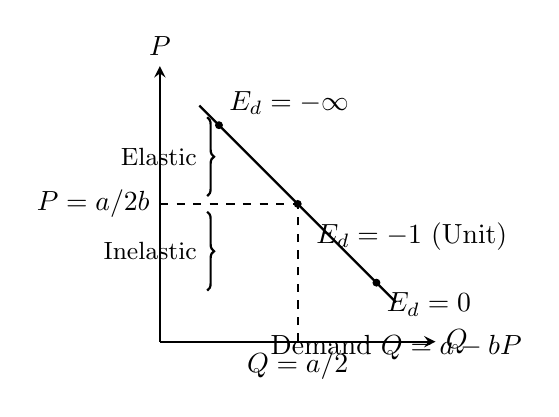
\begin{tikzpicture}[scale=0.5, thick, >=stealth]
    \draw[->] (0,0) -- (7,0) node[right] {$Q$};
    \draw[->] (0,0) -- (0,7) node[above] {$P$};
    \draw[thick] (1,6) -- (6,1) node[below=8pt] {Demand $Q=a-bP$};
    \filldraw (1.5,5.5) circle (2pt) node[above right] {$E_d = -\infty$};
    \filldraw (3.5,3.5) circle (2pt) node[below right=3pt] {$E_d = -1$ (Unit)};
    \filldraw (5.5,1.5) circle (2pt) node[below right] {$E_d = 0$};
    \draw[decorate, decoration=brace] (1.2,5.7) -- (1.2,3.7) node[midway, left] {\small Elastic};
    \draw[decorate, decoration=brace] (1.2,3.3) -- (1.2,1.3) node[midway, left] {\small Inelastic};
    \draw[dashed] (3.5,0) node[below] {$Q=a/2$} -- (3.5,3.5);
    \draw[dashed] (0,3.5) node[left] {$P=a/2b$} -- (3.5,3.5);
\end{tikzpicture}
\end{center}
\textit{Interpretation:} On a straight-line demand curve, elasticity declines as we move down. Upper half: elastic ($|E_d|>1$); Midpoint: unit elastic ($|E_d|=1$); Lower half: inelastic ($0<|E_d|<1$). At vertical intercept, $E_d = -\infty$; at horizontal intercept, $E_d = 0$.

\subsection*{Perfectly Elastic vs. Perfectly Inelastic Demand}
\begin{center}
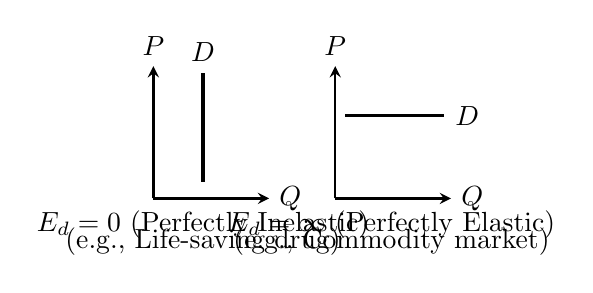
\begin{tikzpicture}[scale=0.42, thick, >=stealth]
    % Perfectly Inelastic
    \draw[->] (0,0) -- (3.5,0) node[right] {$Q$};
    \draw[->] (0,0) -- (0,4) node[above] {$P$};
    \draw[very thick] (1.5,0.5) -- (1.5,3.8) node[above] {$D$};
    \node at (1.5,-0.8) {$E_d = 0$ (Perfectly Inelastic)};
    \node at (1.5,-1.3) {(e.g., Life-saving drug)};
    % Perfectly Elastic
    \draw[->] (5.5,0) -- (9,0) node[right] {$Q$};
    \draw[->] (5.5,0) -- (5.5,4) node[above] {$P$};
    \draw[very thick] (5.8,2.5) -- (8.8,2.5) node[right] {$D$};
    \node at (7.2,-0.8) {$E_d = \infty$ (Perfectly Elastic)};
    \node at (7.2,-1.3) {(e.g., Commodity market)};
\end{tikzpicture}
\end{center}

\subsection*{Total Revenue and Elasticity Relationship}
\begin{center}
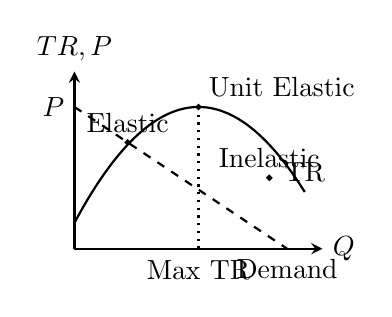
\begin{tikzpicture}[scale=0.45, thick, >=stealth]
    \draw[->] (0,0) -- (7,0) node[right] {$Q$};
    \draw[->] (0,0) -- (0,5) node[above] {$TR, P$};
    % TR curve (inverted U)
    \draw[thick, domain=0:6.5, smooth] plot (\x, {4 - 0.8*(\x-3.5)*(\x-3.5)/3}) node[above] {TR};
    \draw[thick, dashed] (0,4) node[left] {$P$} -- (6,0) node[below] {Demand};
    \filldraw (1.5,3) circle (1.5pt) node[above] {Elastic};
    \filldraw (3.5,4) circle (1.5pt) node[above right] {Unit Elastic};
    \filldraw (5.5,2) circle (1.5pt) node[above] {Inelastic};
    \draw[dotted] (3.5,0) -- (3.5,4);
    \node at (3.5,-0.6) {Max TR};
\end{tikzpicture}
\end{center}
\textit{TR Curve:} Total Revenue ($P \times Q$) reaches maximum at the midpoint (unit elastic point) of a linear demand curve.

% ============================================================================
% PART 5: CALCULATION PROBLEMS AND TECHNIQUES
% ============================================================================
\section*{5. Computing Elasticity -- Detailed Worked Examples}

\subsection*{Example 1: Point Elasticity from Demand Function}
\textbf{Given:} $Q_d = 200 - 4P$. Find $E_d$ at $P = 30$.

\textbf{Solution:}
\begin{enumerate}[leftmargin=*,nosep]
    \item At $P=30$, $Q = 200 - 4(30) = 200 - 120 = 80$.
    \item Derivative: $dQ/dP = -4$.
    \item Point elasticity: $E_d = \frac{dQ}{dP} \cdot \frac{P}{Q} = -4 \cdot \frac{30}{80} = -4 \cdot 0.375 = \mathbf{-1.5}$.
    \item Interpretation: $|E_d| = 1.5 > 1$, demand is \textbf{elastic}. A 1\% price increase leads to a 1.5\% decrease in quantity demanded.
\end{enumerate}

\subsection*{Example 2: Arc Elasticity Calculation}
\textbf{Given:} Price rises from \$10 to \$15, quantity demanded falls from 50 to 30 units.

\textbf{Solution:}
\[
E_d = \frac{(30 - 50) / ((50+30)/2)}{(15 - 10) / ((10+15)/2)} = \frac{-20 / 40}{5 / 12.5} = \frac{-0.5}{0.4} = \mathbf{-1.25}
\]
Interpretation: Over this range, demand is elastic.

\subsection*{Example 3: Income Elasticity from Family Budget Data}
\textbf{Given:} A household's monthly expenditure on meat rises from \$80 to \$96 when monthly income rises from \$2,000 to \$2,400. Calculate income elasticity.

\textbf{Solution:}
\begin{itemize}[leftmargin=*,nosep]
    \item \%$\Delta Q$ = $\frac{96-80}{(96+80)/2} \times 100 = \frac{16}{88} \times 100 = 18.18\%$
    \item \%$\Delta Y$ = $\frac{2400-2000}{(2400+2000)/2} \times 100 = \frac{400}{2200} \times 100 = 18.18\%$
    \item $E_Y = \frac{18.18\%}{18.18\%} = \mathbf{1.0}$ (Unit income elastic -- borderline luxury/necessity).
\end{itemize}

\subsection*{Example 4: Cross Elasticity}
\textbf{Given:} When price of coffee rises from \$4 to \$5 per cup, daily sales of tea increase from 100 to 130 cups. Find $E_{xy}$.

\textbf{Solution:}
\[
\%\Delta Q_{\text{tea}} = \frac{130-100}{(130+100)/2} \times 100 = \frac{30}{115} \times 100 \approx 26.09\%
\]
\[
\%\Delta P_{\text{coffee}} = \frac{5-4}{(5+4)/2} \times 100 = \frac{1}{4.5} \times 100 \approx 22.22\%
\]
\[
E_{xy} = \frac{26.09}{22.22} \approx \mathbf{1.17}
\]
Interpretation: Positive cross elasticity confirms tea and coffee are \textbf{substitutes}. A 1\% rise in coffee price increases tea demand by 1.17\%.

\columnbreak

% ============================================================================
% PART 6: TOTAL REVENUE AND CONSUMER EXPENDITURE PATTERN
% ============================================================================
\section*{6. Elasticity, Total Revenue \& Consumer Expenditure}

\subsection*{The Revenue Test}
Total Revenue ($TR$) = Price $\times$ Quantity = $P \times Q$. The relationship between price change and $TR$ change depends entirely on demand elasticity:

\begin{center}
\begin{tabular}{@{}p{1.5cm}p{2.2cm}p{2.2cm}@{}}
\toprule
\textbf{Elasticity} & \textbf{$P \uparrow$ Effect on $TR$} & \textbf{$P \downarrow$ Effect on $TR$} \\
\midrule
Elastic ($|E_d|>1$) & $TR \downarrow$ & $TR \uparrow$ \\
Unit Elastic ($|E_d|=1$) & $TR$ unchanged & $TR$ unchanged \\
Inelastic ($|E_d|<1$) & $TR \uparrow$ & $TR \downarrow$ \\
\bottomrule
\end{tabular}
\end{center}

\subsection*{Mathematical Proof}
Let $TR = P \cdot Q(P)$. Differentiating with respect to $P$:
\[
\frac{d(TR)}{dP} = Q + P \cdot \frac{dQ}{dP} = Q \left(1 + \frac{P}{Q} \cdot \frac{dQ}{dP}\right) = Q (1 + E_d)
\]
Since $E_d < 0$:
\begin{itemize}[leftmargin=*,nosep]
    \item If $|E_d| > 1$, then $(1+E_d) < 0$, so $d(TR)/dP < 0$: $TR$ falls when $P$ rises.
    \item If $|E_d| < 1$, then $(1+E_d) > 0$, so $d(TR)/dP > 0$: $TR$ rises when $P$ rises.
    \item If $|E_d| = 1$, then $(1+E_d) = 0$, so $d(TR)/dP = 0$: $TR$ is maximized.
\end{itemize}

\subsection*{Consumer Expenditure Pattern}
Consumer expenditure ($E$) on a good = $P \times Q_d$. For normal goods, as price falls, expenditure may rise or fall depending on elasticity:
\begin{itemize}[leftmargin=*,nosep]
    \item \textbf{Elastic goods:} Price cut $\to$ expenditure rises (people buy proportionally more).
    \item \textbf{Inelastic goods:} Price cut $\to$ expenditure falls (people buy only slightly more).
\end{itemize}
This is critical for business pricing strategy: for products with many substitutes (elastic), lowering price increases total sales revenue; for necessities with few alternatives (inelastic), raising price may increase revenue.

\subsection*{Income-Expenditure Patterns (Engel Curve)}
From family budget data, the \textbf{Engel curve} shows relationship between income and expenditure on a good:
\begin{itemize}[leftmargin=*,nosep]
    \item $E_Y > 1$: Share of budget spent on good rises with income (luxuries, e.g., leisure travel).
    \item $0 < E_Y < 1$: Share falls (necessities, e.g., staple food).
    \item $E_Y < 0$: Absolute expenditure falls (inferior goods, e.g., public transport as income rises).
\end{itemize}

% ============================================================================
% PART 7: DETERMINANTS OF ELASTICITY
% ============================================================================
\section*{7. Determinants of Price Elasticity of Demand}

\begin{enumerate}[leftmargin=*,nosep]
    \item \textbf{Availability of Substitutes:} More close substitutes $\to$ higher elasticity (Butter vs. margarine = elastic; Insulin = inelastic). \textit{Most important determinant.}
    \item \textbf{Necessity vs. Luxury:} Necessities (food, water, electricity) tend to be inelastic; luxuries (jewelry, vacation) are elastic.
    \item \textbf{Proportion of Income Spent:} Goods consuming a large fraction of income (housing, cars) are more elastic; small-ticket items (salt, matches) are inelastic.
    \item \textbf{Definition of Market (Breadth):}
    \begin{itemize}[nosep]
        \item Narrowly defined goods (specific brand of rice) have higher elasticity (many substitutes).
        \item Broadly defined categories (all food) have lower elasticity (few substitutes).
    \end{itemize}
    \item \textbf{Time Horizon:} Demand becomes \textbf{more elastic} over time as consumers find alternatives and adjust behavior (short-run gasoline demand is inelastic; long-run, people buy fuel-efficient cars, use transit).
    \item \textbf{Addiction / Habit Formation:} Addictive goods (tobacco, alcohol) tend to have low price elasticity.
    \item \textbf{Durability:} Durable goods (refrigerators, cars) have more elastic demand because purchase can be postponed.
\end{enumerate}

\subsection*{Determinants of Price Elasticity of Supply}
\begin{enumerate}[leftmargin=*,nosep]
    \item \textbf{Time Period:} The most critical factor. \textbf{Momentary supply} (fixed, perfectly inelastic); \textbf{Short-run} (some factors variable, moderately elastic); \textbf{Long-run} (all factors variable, highly elastic).
    \item \textbf{Flexibility of Production:} If resources can be easily shifted in/out (e.g., garment manufacturing), supply is elastic. If specialized capital is needed (e.g., shipbuilding), supply is inelastic.
    \item \textbf{Availability of Inputs:} If inputs are readily available, supply is more elastic.
    \item \textbf{Storage Capacity:} Goods that can be stored cheaply (non-perishables) have more elastic supply; perishables (fresh produce) have inelastic supply.
    \item \textbf{Complexity of Production:} Simple products (textiles) = elastic supply; complex products requiring highly skilled labor (semiconductors) = inelastic supply in short-run.
\end{enumerate}

% ============================================================================
% PART 8: EXTENSIVE CASE STUDIES
% ============================================================================
\section*{8. Comprehensive Case Studies}

\subsection*{Case Study 1: OPEC Oil Price Shocks and the Elasticity of Oil Demand (1973--2023)}

\textbf{Background:} The Organization of Petroleum Exporting Countries (OPEC) is a cartel that controls roughly 40\% of global crude oil production. Understanding the price elasticity of oil demand has been central to predicting cartel power.

\textbf{The 1973 Oil Embargo:} OPEC (Arab members) imposed an oil embargo, sharply cutting supply. Oil prices quadrupled from \$3/barrel to nearly \$12/barrel.

\textbf{Economic Analysis Using Elasticity:}

\textit{Short-Run (1973--1975):}
\begin{itemize}[leftmargin=*,nosep]
    \item \textbf{Demand was highly inelastic ($|E_d| \approx 0.05$ to $0.1$).}
    \item Reasons: No immediate substitutes for gasoline and heating oil; existing stock of cars and furnaces was fuel-inefficient; commuting patterns and housing locations were fixed.
    \item \textbf{Result:} The massive price rise led to only a small decrease in consumption. OPEC revenues soared. The world experienced stagflation -- a supply shock combined with inelastic demand meant high prices without immediate demand adjustment.
\end{itemize}

\textit{Long-Run (1975--1985):}
\begin{itemize}[leftmargin=*,nosep]
    \item \textbf{Demand became more elastic ($|E_d| \approx 0.3$ to $0.5$).}
    \item Reasons: Consumers switched to fuel-efficient Japanese cars; governments mandated Corporate Average Fuel Economy (CAFE) standards; industries adopted energy-saving technologies; home insulation improved; alternative energy (nuclear, coal) expanded.
    \item \textbf{Result:} Oil consumption fell significantly. OPEC's market share and revenue collapsed by the mid-1980s. The price fell below \$10/barrel.
\end{itemize}

\textit{Modern Period (2008--2023):}
\begin{itemize}[leftmargin=*,nosep]
    \item Oil prices spiked to \$147/barrel in 2008, then crashed. The development of fracking technology (shale oil) dramatically increased \textbf{supply elasticity} from non-OPEC sources -- the US became the world's largest producer.
    \item \textbf{Cross-elasticity in action:} Rising oil prices accelerated adoption of electric vehicles (Tesla). EVs are a \textbf{substitute} for gasoline cars. The cross-elasticity of EV demand with respect to gasoline prices is positive and significant ($E_{xy} \approx 0.2$ to $0.4$).
    \item \textbf{2022 Energy Crisis (Russia-Ukraine War):} European natural gas prices surged 5--10 times. Short-run demand for gas was inelastic (winter heating, fixed infrastructure), causing massive expenditure increases for households and industries. Long-run, Europe accelerated renewables and LNG terminals.
\end{itemize}

\textbf{Policy Lesson:} The elasticity of demand determines the effectiveness and consequences of supply shocks. A cartel's long-run power is limited by the long-run demand elasticity being substantially higher than short-run elasticity. Tax/subsidy policies on energy must consider these elasticity dynamics.

\subsection*{Case Study 2: The ``Sin Tax'' -- Cigarette Taxation and Price Elasticity of Demand}

\textbf{Background:} Governments worldwide impose high excise taxes on cigarettes with two objectives: (a) reduce smoking (public health) and (b) raise tax revenue. The effectiveness depends critically on the \textbf{price elasticity of cigarette demand}.

\textbf{The Economic Puzzle:} If demand is inelastic, taxes raise substantial revenue but don't reduce smoking much. If elastic, taxes reduce smoking effectively but raise less revenue. Which is it?

\textbf{Empirical Evidence:}
\begin{itemize}[leftmargin=*,nosep]
    \item \textbf{Adult smokers:} Meta-analyses (Becker, Grossman, Chaloupka) show long-run price elasticity of cigarette demand for adults is approximately $-0.4$ to $-0.6$ (inelastic). A 10\% price increase reduces consumption by 4--6\%.
    \item \textbf{Youth/Teens:} Price elasticity is significantly higher, around $-1.0$ to $-1.4$ (elastic). Young smokers are more price-sensitive due to lower disposable income and less addiction.
    \item \textbf{Income Elasticity:} Cigarettes are an \textbf{inferior good} in developed countries ($E_Y < 0$). As incomes rise, smoking prevalence declines. In developing countries, $E_Y$ may be positive initially.
\end{itemize}

\textbf{Case Study: Australia's Plain Packaging and Tax Hike (2012--2020):}
\begin{itemize}[leftmargin=*,nosep]
    \item Australia imposed plain packaging and raised excise tax annually by 12.5\% (above inflation) from 2013 to 2020. A pack of 25 cigarettes rose from AUD 16 to over AUD 40.
    \item \textbf{Result:} Smoking prevalence fell from 16.1\% (2011--12) to 11.0\% (2019). Daily smokers declined. Government tobacco excise revenue continued to rise despite falling volume because demand is inelastic -- the \textbf{revenue effect} outweighed the quantity effect. Revenue rose from AUD 8.3 billion (2012) to over AUD 17 billion (2019).
    \item \textbf{Deadweight Loss:} Because demand is relatively inelastic, the deadweight loss per dollar of tax raised is smaller than for elastic goods -- making it a relatively ``efficient'' tax from a welfare perspective.
    \item \textbf{Regressive Impact:} Smoking prevalence is higher among lower-income groups. Because demand is inelastic among addicted low-income smokers, the tax burden falls disproportionately on them, raising equity concerns.
    \item \textbf{Illicit Trade:} High taxes create incentives for black market cigarettes. Elasticity of supply of illicit tobacco (highly elastic, mobile) partially offsets the health gains. Australia's extensive border controls limited this.
\end{itemize}

\textbf{Policy Design Implications:}
\begin{enumerate}[leftmargin=*,nosep]
    \item Since youth demand is elastic, price increases are particularly effective at preventing smoking initiation -- a major public health win.
    \item For addicted adult smokers (inelastic demand), complementary policies (cessation support, nicotine replacement therapy) are needed alongside taxes.
    \item Revenue from sin taxes can hypothetically fund health programs, but governments may become dependent on this revenue stream.
    \item Cross-elasticity: As cigarette prices rise, demand for substitutes like e-cigarettes/vaping increases (positive cross-elasticity), creating new regulatory challenges.
\end{enumerate}

\textbf{Economic Concept Summary:} The case demonstrates the power of elasticity analysis in policy -- understanding \textbf{who responds, by how much, and over what time horizon} is essential for predicting outcomes of taxation and designing effective, equitable interventions.

% ============================================================================
% PART 9: EXAM QUESTIONS WITH MODEL ANSWERS
% ============================================================================
\section*{9. Exam Practice Questions \& Detailed Answers}

\subsection*{Question 1: Calculation (Comprehensive)}
\textbf{The demand for a product is given by $Q_d = 500 - 0.5P$.}
\textbf{(a) Find price elasticity at $P = 400$ and $P = 600$. Interpret.}
\textbf{(b) At what price is demand unit elastic?}
\textbf{(c) If the current price is \$400, should the firm raise or lower price to increase total revenue? Explain using elasticity and the total revenue test.}
\textbf{(d) If consumer income increases by 10\% and demand becomes $Q_d = 560 - 0.5P$, calculate the income elasticity of demand at the original price of \$400. Classify the good.}

\vspace{0.1cm}
\textbf{Model Solution:}
\vspace{0.05cm}
\textbf{(a)} $dQ/dP = -0.5$.
\begin{itemize}[nosep]
    \item At $P=400$: $Q = 500 - 0.5(400) = 300$. $E_d = -0.5 \times \frac{400}{300} = -0.667$. $|E_d| = 0.667 < 1$. Demand is \textbf{inelastic}.
    \item At $P=600$: $Q = 500 - 0.5(600) = 200$. $E_d = -0.5 \times \frac{600}{200} = -1.5$. $|E_d| = 1.5 > 1$. Demand is \textbf{elastic}.
\end{itemize}
\textbf{(b)} Unit elastic when $|E_d| = 1$:
$| -0.5 \times \frac{P}{500 - 0.5P} | = 1 \implies 0.5P = 500 - 0.5P \implies P = 500$. At $P=500$, $Q=250$.

\textbf{(c)} At $P=400$, $|E_d| = 0.667 < 1$ (inelastic). With inelastic demand, a price \textbf{increase} will raise Total Revenue ($TR$). $TR$ currently = $400 \times 300 = 120,000$. If $P$ rose to e.g., \$500, $Q=250$, $TR = 125,000$ (higher). The firm should \textbf{raise price}.

\textbf{(d)} At $P=400$, original $Q_1 = 300$, new $Q_2 = 560 - 0.5(400) = 360$.
$\%\Delta Q = \frac{360-300}{(360+300)/2} \times 100 = \frac{60}{330} \times 100 \approx 18.18\%$. $\%\Delta Y = 10\%$.
$E_Y = \frac{18.18}{10} \approx 1.82$. Since $E_Y > 0$ and $> 1$, the good is a \textbf{luxury normal good}.

\vspace{0.2cm}

\subsection*{Question 2: Conceptual Application}
\textbf{Suppose the government imposes a tax on sugary drinks to reduce obesity. Using the concepts of price elasticity of demand and cross-elasticity, explain:}
\textbf{(a) Why the effectiveness of the tax depends on the own-price elasticity of sugary drinks.}
\textbf{(b) Why we must also consider the cross-elasticity with non-sugary drinks and other snacks.}
\textbf{(c) How the tax incidence between consumers and producers relates to elasticity.}

\vspace{0.1cm}
\textbf{Answer:}
\vspace{0.05cm}
\textbf{(a) Effectiveness depends on $E_d$:} The tax raises the price of sugary drinks. The reduction in consumption equals \%$\Delta P \times E_d$. If demand is elastic ($|E_d| > 1$), the quantity consumed falls substantially, achieving health goals. If demand is inelastic ($|E_d| < 1$, e.g., due to addiction/habit), consumption falls only modestly, and the tax primarily raises revenue without significantly changing behavior. Evidence suggests sugary drink demand is moderately elastic ($|E_d| \approx 1.0 - 1.3$), so taxes can be effective.

\textbf{(b) Cross-elasticity matters:} Consumers may substitute away from taxed sugary drinks to \textbf{untaxed alternatives}. If cross-elasticity with diet drinks is positive and high ($E_{xy} \gg 0$), consumers switch to diet sodas -- a positive health outcome. However, if cross-elasticity with other unhealthy goods like sugary snacks or fruit juices (high in natural sugar) is also positive, the net health benefit may be smaller. Cross-elasticity with \textbf{bottled water} is an important policy parameter. If water is a close substitute (high $+E_{xy}$), the tax may have a double benefit -- reduced soda, increased water consumption.

\textbf{(c) Tax incidence:} The burden of the tax falls more heavily on the side of the market that is \textbf{less elastic}. If demand for sugary drinks is relatively inelastic compared to supply, consumers bear most of the tax through higher prices. If supply is inelastic (e.g., limited bottling capacity in short-run), producers bear more. Empirical evidence suggests consumer demand is more inelastic than producer supply (especially given many beverage alternatives in supply), meaning consumers pay the majority of a soda tax.

\vspace{0.2cm}

\subsection*{Question 3: Data Analysis}
\textbf{A household's monthly budget at two income levels is given. Analyze income elasticity and classify each good.}

\begin{center}
\begin{tabular}{@{}lcc@{}}
\toprule
\textbf{Good} & \textbf{Income =\$3,000} & \textbf{Income =\$4,500} \\
\midrule
Food (total) & \$900 & \$1,200 \\
Public Transport & \$200 & \$180 \\
Entertainment & \$150 & \$360 \\
\bottomrule
\end{tabular}
\end{center}

\textbf{Solution:}
\begin{itemize}[leftmargin=*,nosep]
    \item \textbf{Food:} $\%\Delta Q = \frac{300}{1050} \times 100 = 28.57\%$; $\%\Delta Y = \frac{1500}{3750} \times 100 = 40\%$. $E_Y = 28.57/40 = 0.714$. ($0 < E_Y < 1$: \textbf{Necessity}).
    \item \textbf{Public Transport:} $\%\Delta Q = \frac{-20}{190} \times 100 = -10.53\%$. $E_Y = -10.53/40 = -0.263$. ($E_Y < 0$: \textbf{Inferior good} -- as income rises, household spends less on buses, may buy a car).
    \item \textbf{Entertainment:} $\%\Delta Q = \frac{210}{255} \times 100 = 82.35\%$. $E_Y = 82.35/40 = 2.06$. ($E_Y > 1$: \textbf{Luxury}).
\end{itemize}

\vspace{0.2cm}

\subsection*{Question 4: Short Conceptual}
\textbf{Explain why the price elasticity of demand for a specific brand of salt is likely much higher than the elasticity of demand for salt as a whole.}

\textbf{Answer:} A specific brand of salt (e.g., ``Tata Salt'') has many close \textbf{substitutes} -- other branded salts, generic store brands, sea salt, rock salt. If Tata raises its price, consumers easily switch to alternatives, so demand is \textbf{elastic}. Salt as a whole (a broad category) has \textbf{no close substitutes} and constitutes a tiny fraction of consumer income; it is a necessity. Therefore, aggregate salt demand is highly \textbf{inelastic} ($|E_d| \approx 0.1$). This illustrates the principle: \textit{The narrower the market definition, the higher the elasticity}.

\end{multicols}

% ============================================================================
% SINGLE COLUMN SUMMARY TABLE
% ============================================================================
\vspace{0.3cm}
\begin{center}
\fbox{\begin{minipage}{0.9\textwidth}
\footnotesize
\textbf{Summary Cheat Sheet: Elasticity Formulae and Sign Conventions}
\begin{center}
\begin{tabular}{@{}p{2.8cm}p{1.8cm}p{2.2cm}p{2.2cm}@{}}
\toprule
\textbf{Elasticity Type} & \textbf{Formula} & \textbf{Sign} & \textbf{Interpretation} \\
\midrule
Price Elasticity ($E_d$) & $\frac{dQ}{dP} \cdot \frac{P}{Q}$ & Negative ($-$) & $|E_d|>1$ elastic; $<1$ inelastic \\
Income Elasticity ($E_Y$) & $\frac{dQ}{dY} \cdot \frac{Y}{Q}$ & $+$ Normal; $-$ Inferior & $>1$ luxury; $0$--$1$ necessity \\
Cross Elasticity ($E_{xy}$) & $\frac{dQ_x}{dP_y} \cdot \frac{P_y}{Q_x}$ & $+$ Substitutes; $-$ Complements & Magnitude shows strength of relationship \\
Supply Elasticity ($E_s$) & $\frac{dQ_s}{dP} \cdot \frac{P}{Q_s}$ & Positive ($+$) & Higher in long-run \\
Arc Elasticity & $\frac{\Delta Q}{\Delta P} \cdot \frac{P_1+P_2}{Q_1+Q_2}$ & (Depends) & Use for discrete/large changes \\
\bottomrule
\end{tabular}
\end{center}

\vspace{0.1cm}
\textbf{Key Relationships to Remember:}
\begin{itemize}[leftmargin=*,nosep]
    \item $TR$ maximized when $|E_d| = 1$; $MR = P(1 + 1/E_d)$. If $|E_d| > 1$, $MR > 0$; if $|E_d| < 1$, $MR < 0$.
    \item Elasticity varies \textit{along} a linear demand curve; constant only for special forms ($Q = aP^{-b}$).
    \item Engel's Law: As income rises, the proportion of income spent on food falls (food income elasticity $< 1$).
\end{itemize}
\end{minipage}}
\end{center}

\end{document}